\section{Generative adapters expose model--interface interaction}
\label{sec:generative}
The historical Llama and Qwen comparisons use a fixed one-forward-pass
candidate-code logit adapter, not free generation. To test whether that choice
drives the conclusions, we froze a prediction-independent, source-balanced
challenge of 212 states from 18 suites spanning all 15 current source
collections. One question per state, its reference, candidate order and full
input are held fixed. CLINC150/OOS is deliberately balanced between six
rejection and six named-intent cases; this is a diagnostic subset, not a
prevalence-weighted benchmark estimate. Each model is evaluated with two
additional zero-shot adapters: greedy direct code generation using the
historical prompt, and greedy generation after a fixed brief-explanation
instruction ending in a final code. The checkpoint and chat-template hashes
match the original baseline. Neither prompted adapter emits calibrated typed
confidence or an ordinal expectation, so this comparison concerns discrete
label accuracy and decision turnover only.

We also froze a smaller, exact-input direct-generation control on the new natural-domain cases: the same 144 legal and 180 three-class scientific requests for each 8B model, with the historical message template, greedy decoding and a strict whole-response one-code parser. All 648 generated answers are valid and have exactly the same semantic label as the corresponding one-forward-pass code-logit outputs; no source-domain accuracy or prediction transition changes under this adapter substitution. Prompt-token hashes and source IDs match the original requests. This rules out a ``single-token scoring versus direct code generation'' discrepancy on these selected cases and this prompt; it does not show that either model's best prompted legal/scientific performance has been reached, or that their probability outputs are equivalent.

\begin{figure}[!t]
\centering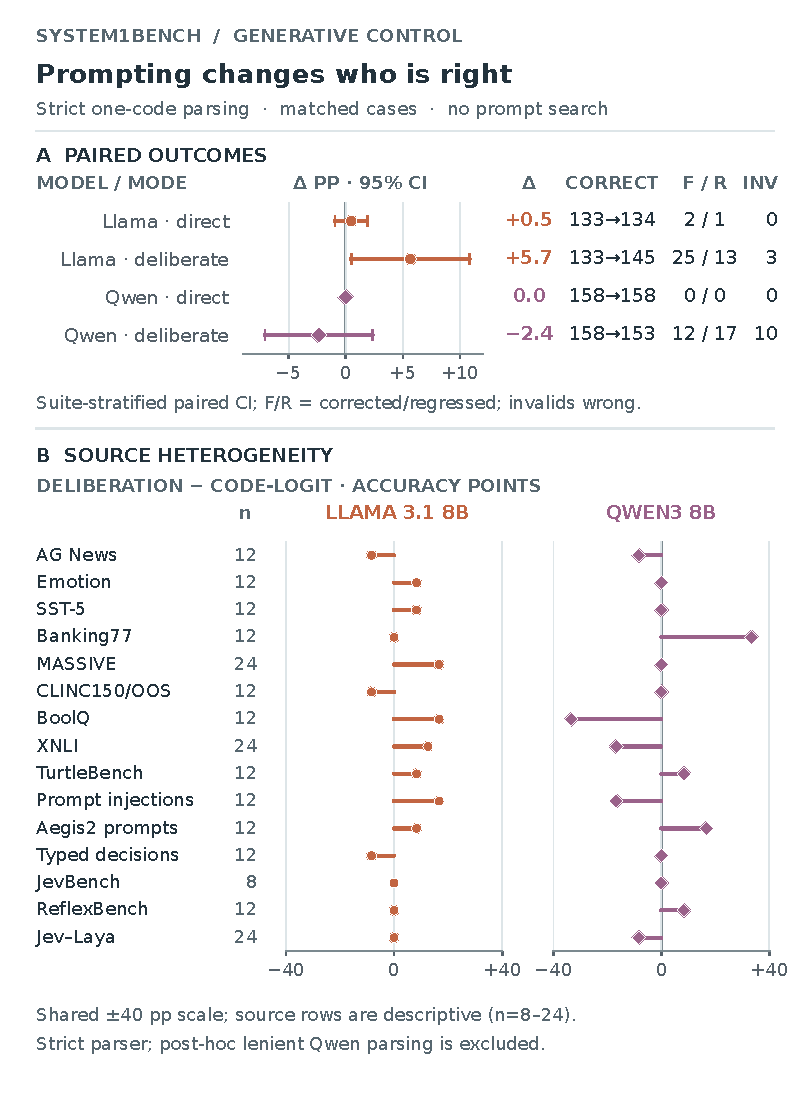
\includegraphics[width=.99\linewidth]{figures/fig_strong_baseline_main.pdf}
\caption{Prompted-baseline stress test on 212 matched states/model. Top:
correction and regression flows, net accuracy effect and 95\% paired
suite-stratified bootstrap interval versus the historical code-logit output.
Bottom: descriptive brief-deliberation effect by source ($n=8$--24), on a
shared percentage-point scale, without per-source significance tests. Invalid generations count incorrect; the
post-hoc parser sensitivity is excluded.}
\label{fig:strong-baseline}
\end{figure}

Figure~\ref{fig:strong-baseline} separates two effects that an aggregate score
would hide. Direct generation changes none of Qwen's 212 predictions and only
five of Llama's, consistent with the historical adapter's constrained
next-token decision on this subset. Brief deliberation changes 55 Llama and
46 Qwen predictions. Llama's correctness rises from 133/212 to 145/212:
25 incorrect decisions are corrected while 13 correct decisions regress,
with three invalid generations. Qwen moves from 158/212 to 153/212:
12 corrections coexist with 17 regressions and ten invalid generations.
The selected-state paired effects are $+5.7$ points (95\% interval
$[+0.5,+10.8]$) and $-2.4$ points ($[-7.1,+2.4]$), respectively. However,
when the 15 sources receive equal weight, Llama's effect is $+4.7$ points
with interval $[-1.4,+10.6]$; a source-general improvement is not established.

The source view makes the interaction more concrete without elevating small
cells into claims of significance. Llama corrects four additional English
XNLI cases but loses one Chinese XNLI case. Qwen corrects four Banking77
cases, whereas four BoolQ answers become invalid under the predeclared
output grammar; its XNLI sample loses four correct answers in 24 states.
These results suggest that prompting is an intervention on a
\emph{model--adapter--task} combination, not an intrinsic improvement
operator for an LLM.

Output validity materially affects the conclusion. Llama's three invalids
hit the 128-token cap before a final code. Eight of Qwen's ten invalids
actually end in an inline \texttt{FINAL:} code rather than the required
standalone final line; two say \texttt{FINAL: None}. A clearly post-hoc
end-of-response parser would recover eight answers, six correct, yielding
159/212 for Qwen instead of the registered 153/212. We retain the strict
result as primary: the sensitivity distinguishes semantic selection from
interface compliance, not permission to tune the evaluator after seeing
answers. Brief deliberation used 87.6/90.1 seconds of synchronized local
generation for Llama/Qwen versus 15.7/16.9 seconds for direct generation
(batch size four, excluding load and tokenization); these implementation
times are not merged with the separate performance experiment. One frozen
128-token prompt cannot bound either model's best prompted performance.
\FloatBarrier
